\section{Hybrid control}
% presentation de la dynamique et hypothèse

\setcounter{subsection}{1}
\begin{frame}{Behavior without the controller}
  \begin{center}
    \vspace*{0.5cm}
    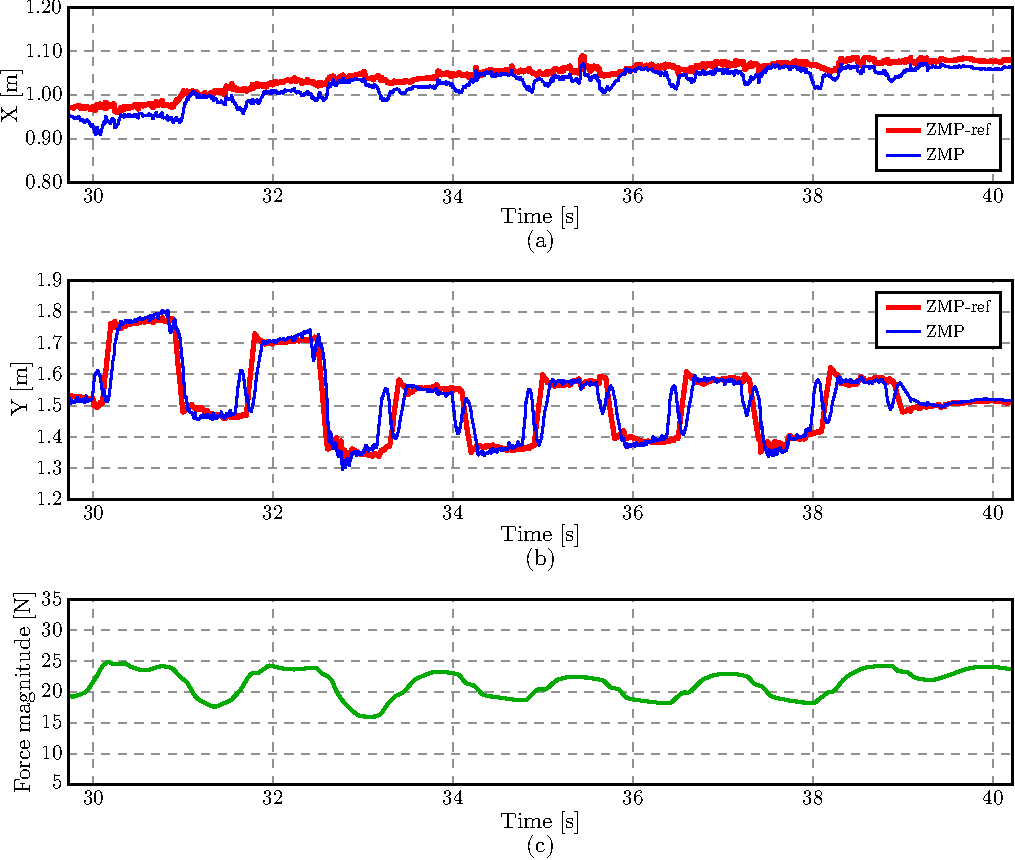
\includegraphics[height=6cm]{hose_xp/exp_ZMP_noCont.pdf}\\
    \textbf{\color{blue} Swing foot bounce once before landing}
  \end{center}
\end{frame}

\begin{frame}{Equation of the controller}
  \vspace*{0.5cm}
  \tikzstyle{na} = [baseline=-.5ex]
  \begin{itemize}
    \item pulling force
      \tikz[na] \node[coordinate] (nfpull) {};
    \item desired force
      \tikz[na] \node[coordinate] (nfd) {};
    \item wrist measured \\external force 
      \tikz[na] \node[coordinate] (nflw) {};
  \end{itemize}
%
  \vspace*{-0.5cm}
  \begin{align*}
    m \tikz[baseline]{
      \node[fill=green!20,anchor=base] (a)
      { $ \ddot{\bf x}_{lw} $ };
    }
   + c \tikz[baseline]{
      \node[fill=green!20,anchor=base] (v)
      {$ \dot{\bf x}_{lw} $};
    } = 
    \tikz[baseline]{
      \node[fill=red!20,anchor=base] (flw)
      {$ {\bf f}_{lw} $};
    } + 
    \tikz[baseline]{
      \node[fill=purple!20,anchor=base] (fd)
      {$ {\bf f}_{d} $};
    } + 
    \tikz[baseline]{
      \node[fill=blue!20,anchor=base] (fpull)
      {$ {\bf f}_{pull} $};
    }
  \end{align*}
  \vspace*{-0.5cm}
  \begin{itemize}
    \item left wrist velocity\\
    and acceleration \tikz[na] \node[coordinate] (nav) {};
  \end{itemize}

{\footnotesize
  $ {\bf x}_{lw} = [x_{lw} , z_{lw}] $ ; m and c chosen empirically ;
  $ \mathbf{f}_{\mathrm{pull}} =
  \begin{cases}
    \mathbf{W} \, \mathbf{v}^{\mathrm{ref}}	& \quad \mathrm{if} \;
    \text{double support}  \\
    0  & \quad \mathrm{otherwise}
  \end{cases}$
}

% Now it's time to draw some edges between the global nodes. Note that we
% have to apply the 'overlay' style.
  \begin{tikzpicture}[overlay]
    \path[->,line width=0.5mm, green!50!black!70]  <2-> (nav) edge [bend right] (a);
    \path[->,line width=0.5mm, green!50!black!70]  <2-> (nav) edge [bend right] (v);
    \path[->,line width=0.5mm, red!100!black!80]   <3-> (nflw) edge [bend left] (flw);
    \path[->,line width=0.5mm, purple!100!black!80]<4-> (nfd) edge [bend left] (fd);
    \path[->,line width=0.5mm, blue!50!black!70]   <5-> (nfpull) edge [bend left] (fpull);
  \end{tikzpicture}



\end{frame}

\begin{frame}{Behavior with the controller}
  \begin{center}
    \vspace*{0.5cm}
    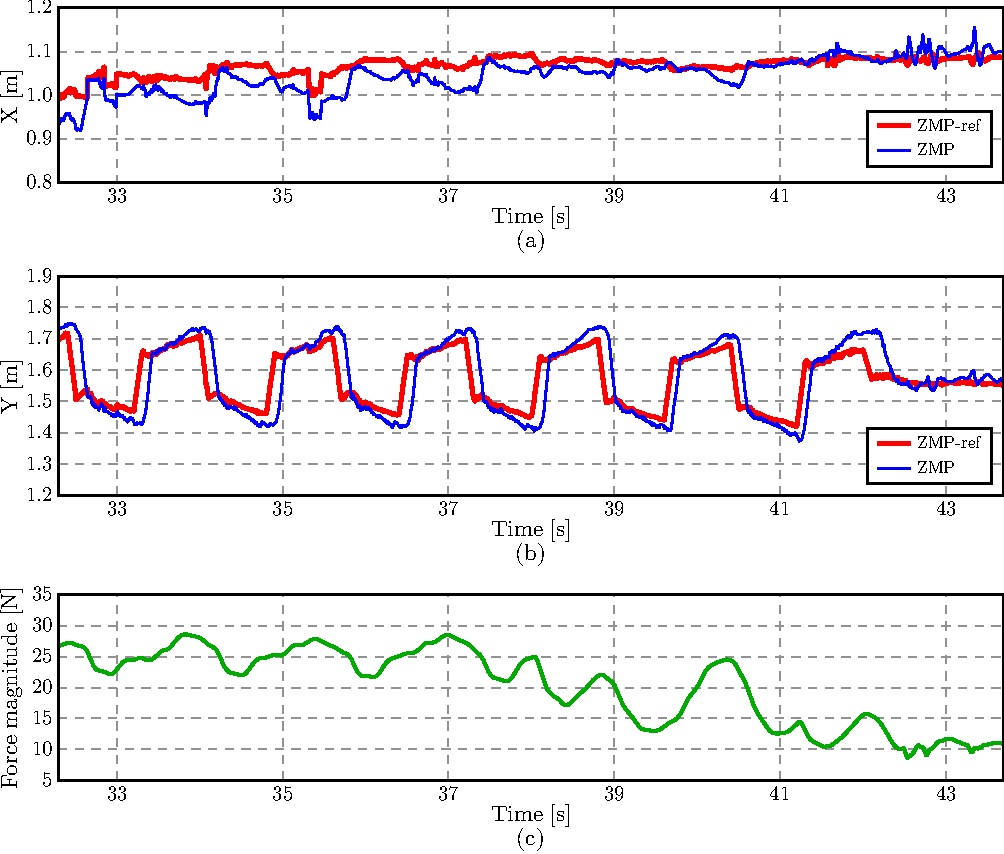
\includegraphics[height=6cm]{hose_xp/exp_ZMP_cont.pdf}\\
    \textbf{\color{blue} No bouncing anymore, $ZMP$ differ in double support due to $ f_{pull}$}
  \end{center}
\end{frame}
